\subsection{Checkout - Shipping Page}

%For the main pages put a mockup and describe it in detail.

%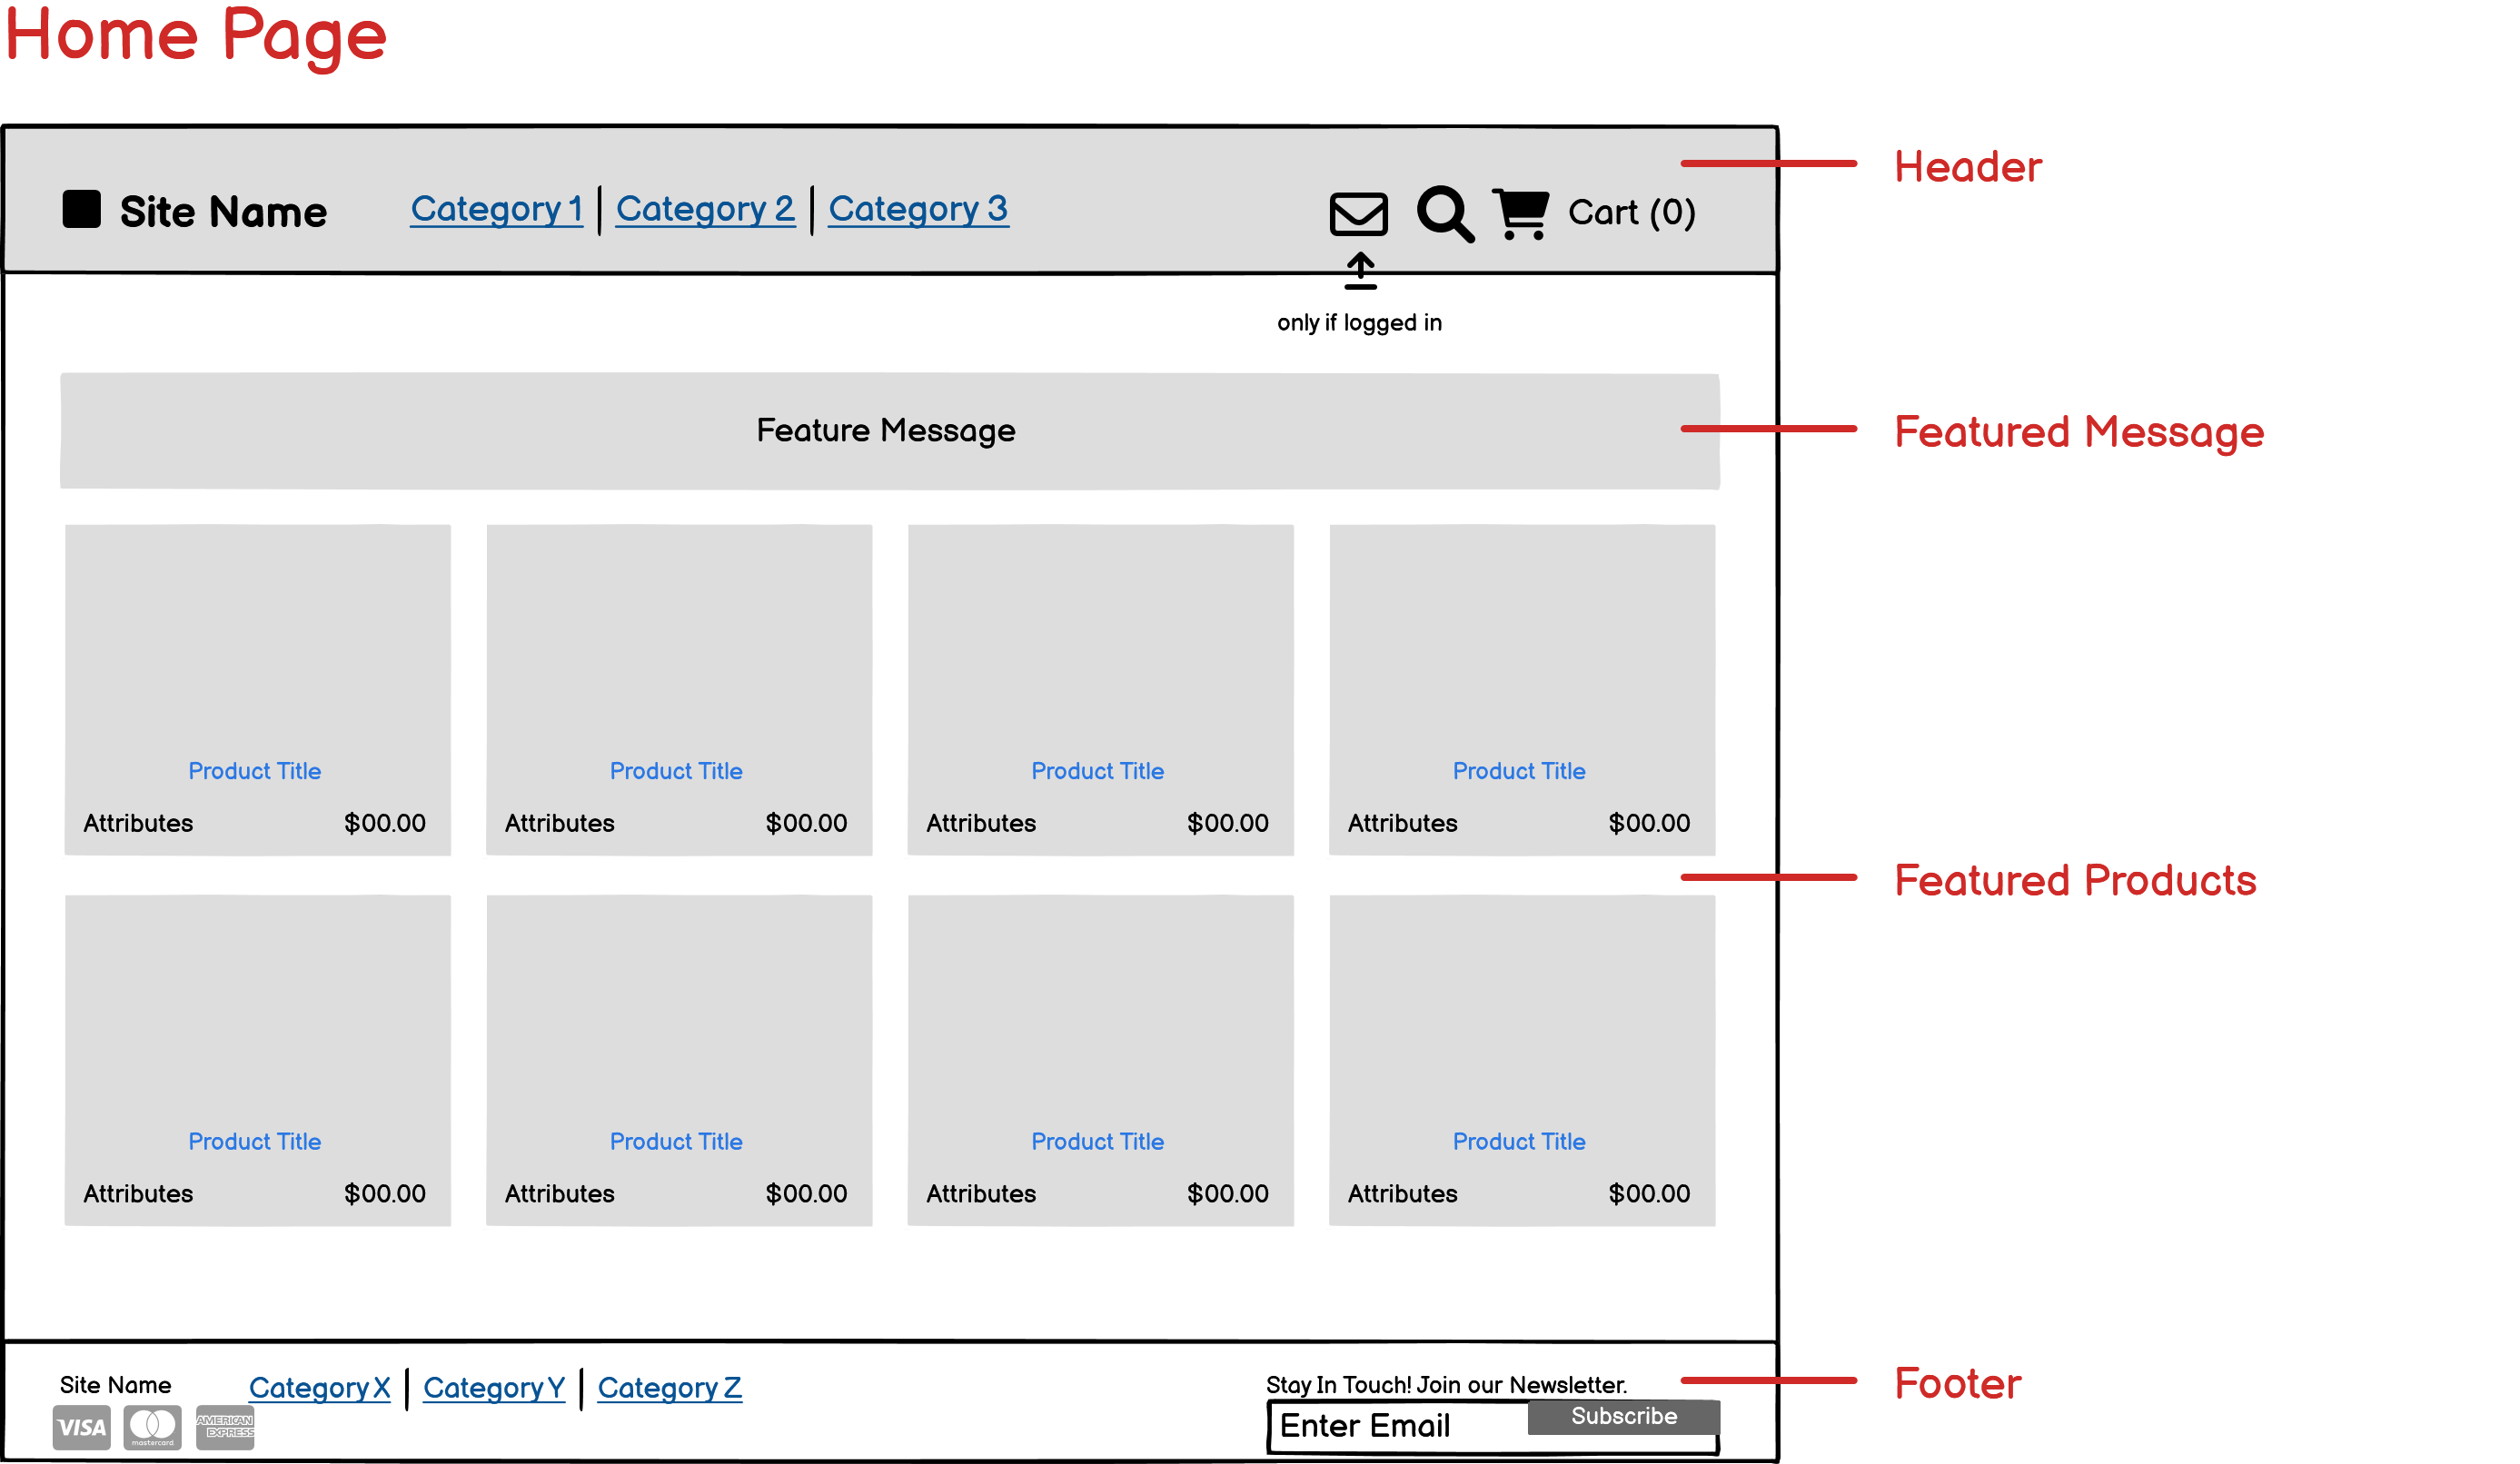
\includegraphics[scale=0.5]{logos/Images/pages/Home Page.png}

\begin{figure}[h]
    \centering
    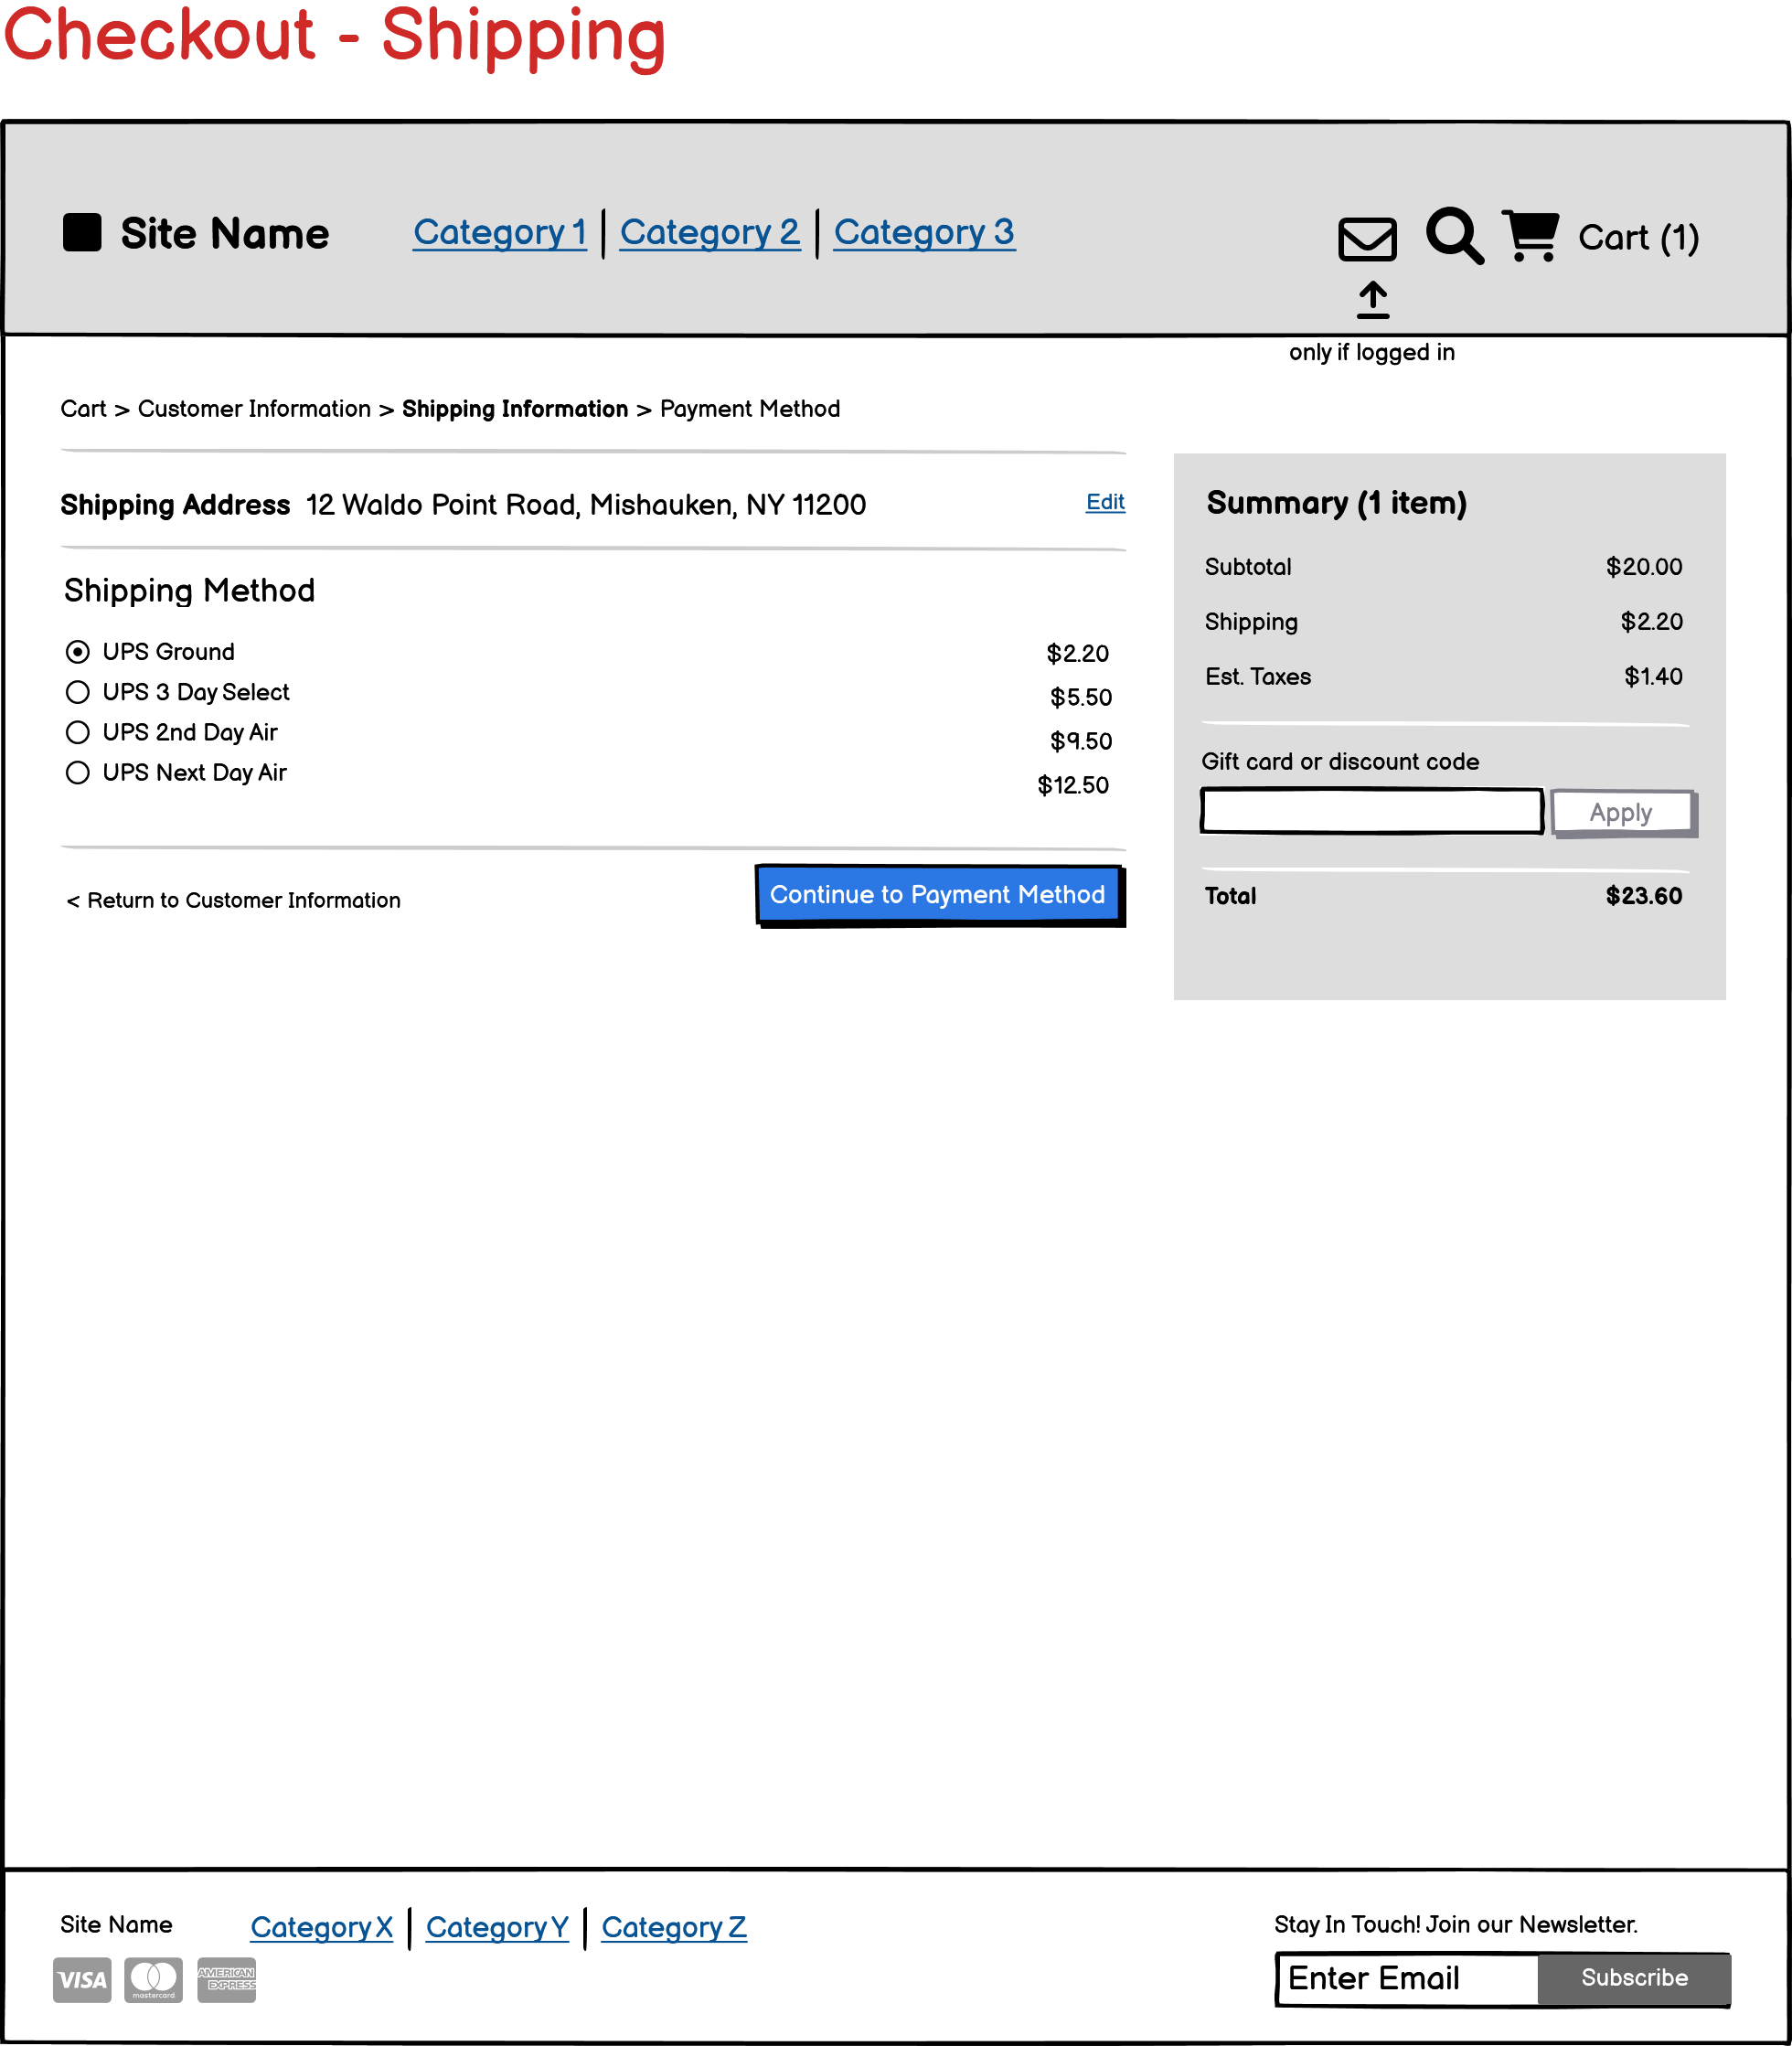
\includegraphics[scale=0.5]{logos/Images/pages/Checkout - Shipping.png}
    \caption{Checkout - Shipping}
    \label{fig:my_label}
\end{figure}
\hfill \break
When a user places an order on this website, they have the option to select the delivery address and delivery service.\\\\
On the left side of the delivery method page, the user can select the delivery address and choose the preferred delivery service from a list of available options. Here the user can also make comments about the delivery or specify special requirements.\\\\
On the right side of the page is an order summary that lists all items purchased, the number of products ordered, and the total price of the order.\\\\
The Delivery Method page provides the user with a quick and easy way to check the details of their order and ensure that the delivery address and delivery service are correct. This way, the user can ensure that their order will be delivered on time and to the correct address.